\documentclass{standalone}
\usepackage{picture,color}
\usepackage{graphicx}
\graphicspath{{./Fig_Striatum_subfigs/}}
\setlength{\unitlength}{1in}
\usepackage{helvet}
\renewcommand{\familydefault}{\sfdefault}

\begin{document}
\begin{picture}(6.85, 6.55)(0,-6.8)
% example frame 
\put(0.22, -1.4){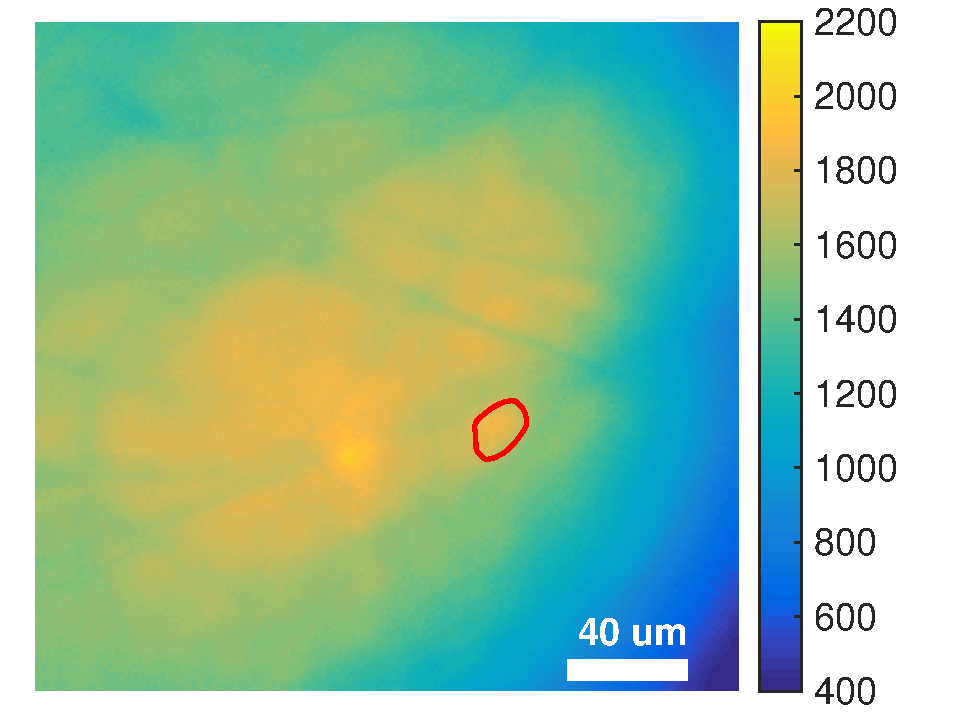
\includegraphics[height=1in]{Fig_Striatum_subfigs/example_frame.pdf}}
\put(0.02, -0.45){\large\textbf{A}}
\put(.47, -0.4){\scriptsize Raw data}

\put(1.45,-0.95){\large\textbf{=}}
\put(1.57, -1.4){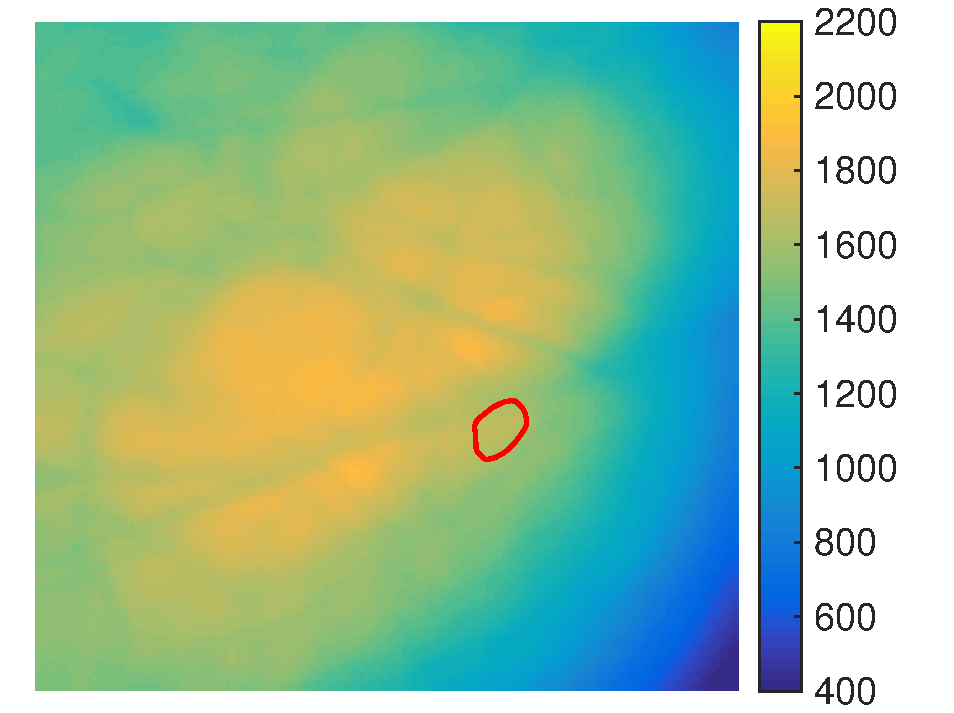
\includegraphics[height=1in]{Fig_Striatum_subfigs/example_frame_bg_constant.pdf}}
\put(1.7, -0.4){\scriptsize Const. baseline}

\put(2.8,-0.95){\large\textbf{+}}
\put(2.92, -1.4){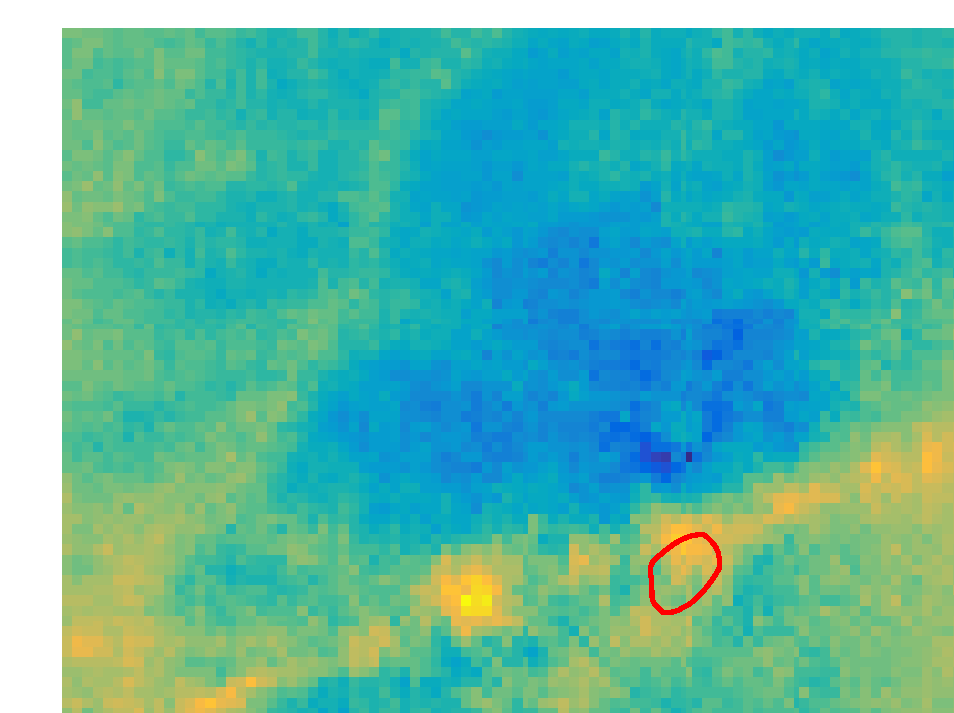
\includegraphics[height=1in]{Fig_Striatum_subfigs/example_frame_bg_fluc.pdf}}
\put(3.01, -0.4){\scriptsize Fluc. background}

\put(4.15,-0.95){\large\textbf{+}}
\put(4.27, -1.4){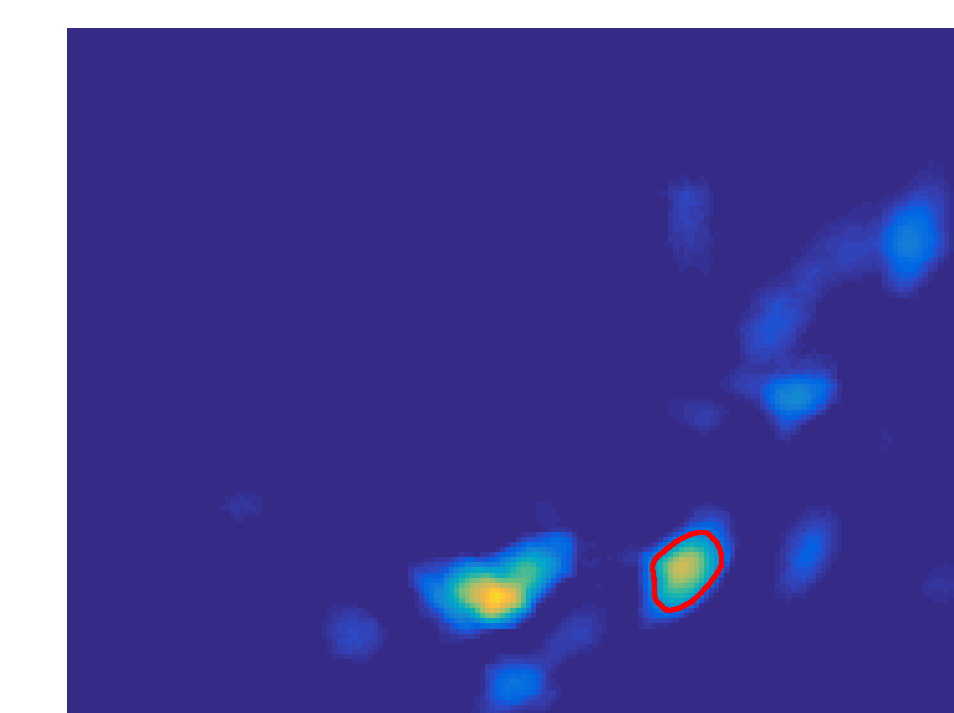
\includegraphics[height=1in]{Fig_Striatum_subfigs/example_frame_ac.pdf}}
\put(4.44, -0.4){\scriptsize Neural signal}

\put(5.50,-0.95){\large\textbf{+}}
\put(5.62, -1.4){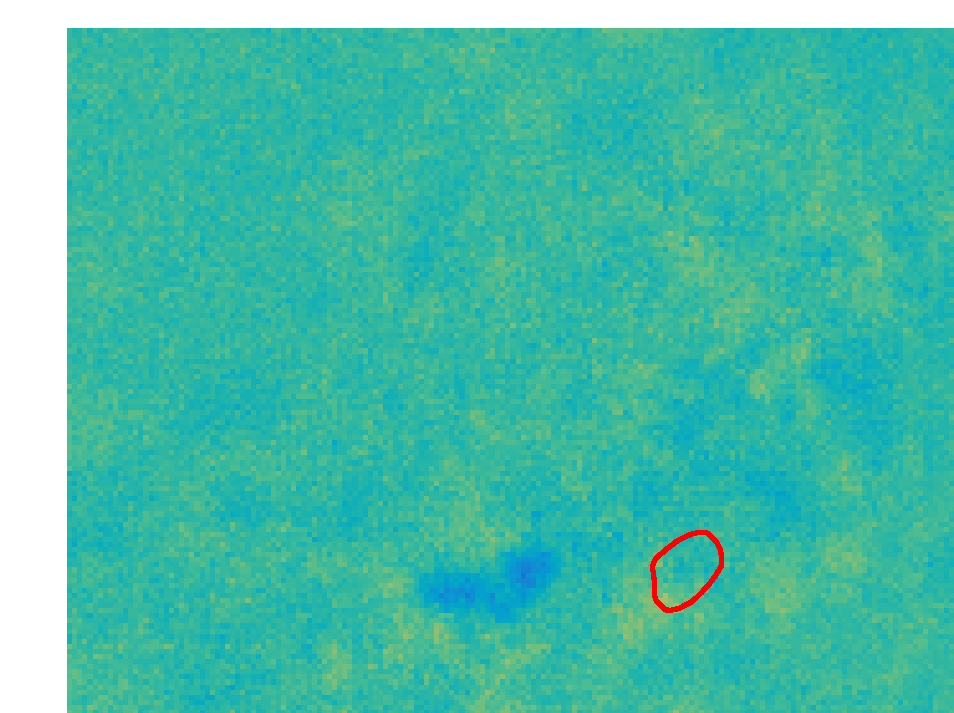
\includegraphics[height=1in]{Fig_Striatum_subfigs/example_frame_res.pdf}}
\put(5.87, -0.4){\scriptsize Residual}

% % traces within an selected ROI 
\put(0.2, -2.9){\includegraphics[height=1.3in]{Fig_Striatum_subfigs/example_roi_traces.pdf}}
\put(0.02, -1.59){\large\textbf{B}}
\put(0.47, -1.53){\scriptsize Fluorescence traces within the ROI}

% contour plot  
\put(4.9, -4.785){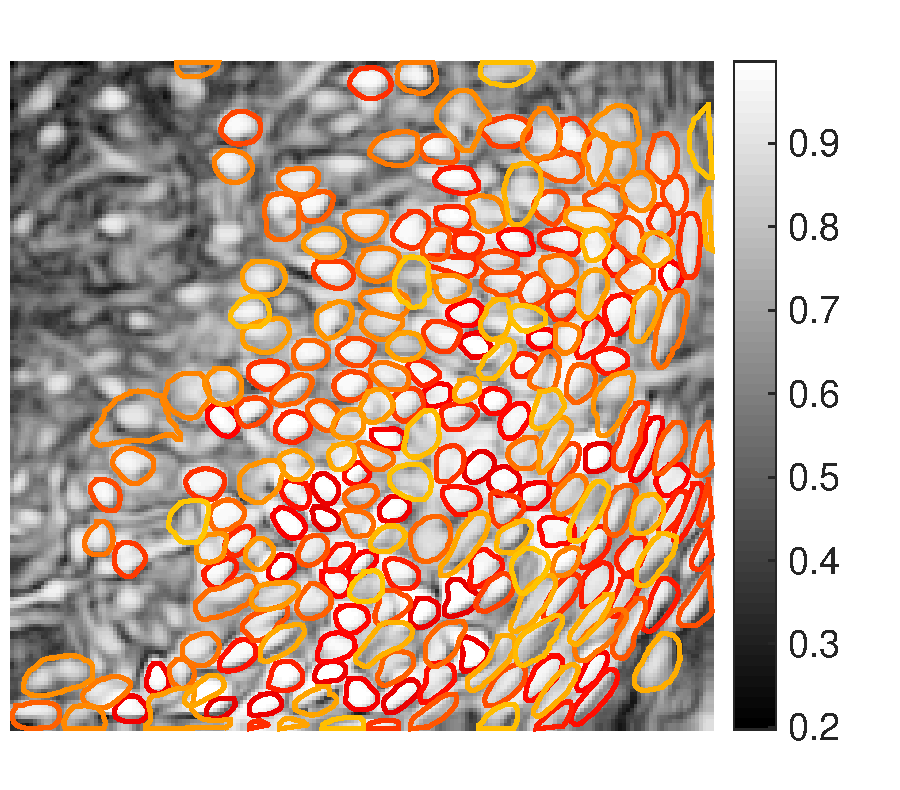
\includegraphics[height=1.58in]{Fig_Striatum_subfigs/contours_ica.pdf}}
\put(4.9, -3.185){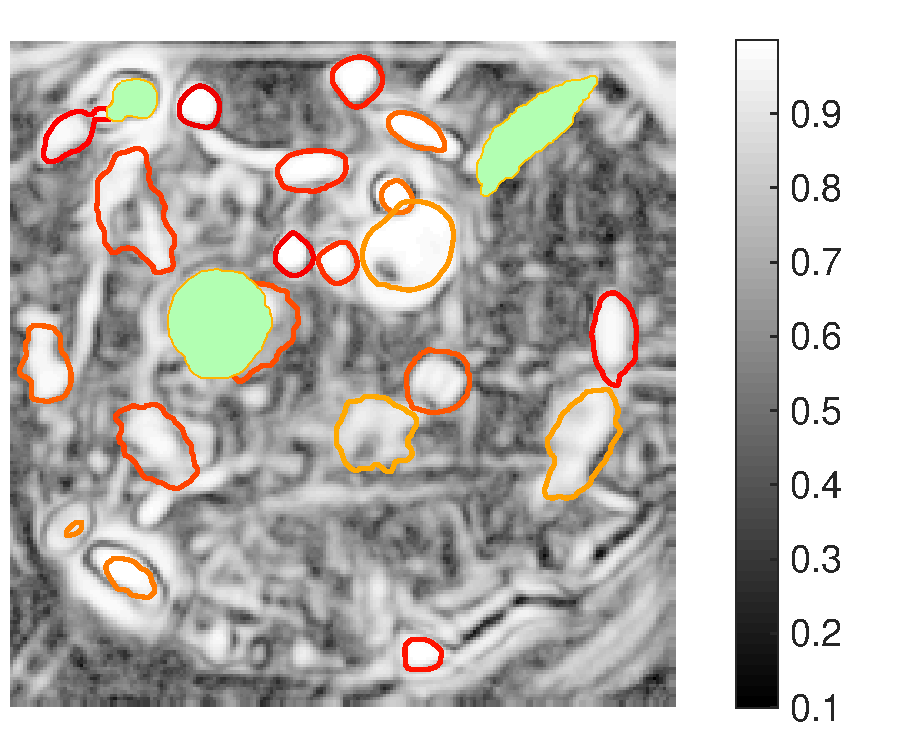
\includegraphics[height=1.58in]{Fig_Striatum_subfigs/contours_cnmfe.pdf}}
\put(4.6, -1.59){\large\textbf{D}}
\put(5.5, -1.53){\scriptsize Contour plot}
\put(4.72, -1.59){\line(1,0){2.08}}
\put(6.8,-1.59){\line(0, -1){3.2}}
\put(4.72, -1.59){\line(0,-1){3.2}}
\put(4.72, -4.79){\line(1,0){2.08}}
\put(4.77, -2.7){\rotatebox{90}{CNMF-E}}
\put(4.77, -4.3){\rotatebox{90}{PCA/ICA}}
% \put(4.82, -3.33){\large\textbf{E}}
% \put(5.27, -3.28){\scriptsize Contour plot}
% \put()

\put(0.28, -3.62){\includegraphics[height=0.32in]{Fig_Striatum_subfigs/ica_missed_spatial.pdf}}
\put(0, -4.95){\includegraphics[height=1.4in]{Fig_Striatum_subfigs/ica_missed_temporal.pdf}}
\put(0.02, -3.33){\large\textbf{E}}
\put(1.5, -3.28){\scriptsize Components detected by CNMF-E only}

\put(0.07, -6.84){\includegraphics[height=1.73in]{Fig_Striatum_subfigs/snr_pca_ica.pdf}}
\put(0.02, -5.13){\large\textbf{F}}
\put(0.67, -5.08){\scriptsize SNR}

% matched neurons 

\put(4.68, -6.75){\includegraphics[height=1.65in]{Fig_Striatum_subfigs/matched_temporal_ica.pdf}}
\put(2.72, -6.75){\includegraphics[height=1.65in]{Fig_Striatum_subfigs/matched_temporal_cnmfe.pdf}}

\put(2.1, -6.85){\includegraphics[height=0.65in]{Fig_Striatum_subfigs/colorbar_ica.pdf}}
\put(1.47, -6.85){\includegraphics[height=0.65in]{Fig_Striatum_subfigs/colorbar_cnmfe.pdf}}

\put(1.5, -6.6){\includegraphics[height=1.5in]{Fig_Striatum_subfigs/match_spatial_cnmfe.pdf}}
\put(2.13, -6.6){\includegraphics[height=1.5in]{Fig_Striatum_subfigs/match_spatial_ICA.pdf}}


\put(1.32, -5.13){\large\textbf{G}}
\put(1.61, -5.08){\scriptsize CNMF-E}
\put(2.26, -5.08){\scriptsize PCA/ICA}

\put(3.5, -5.08){\scriptsize CNMF-E traces}
\put(5.45, -5.08){\scriptsize PCA/ICA traces}
% \put(1.9, -5.03){\large\textbf{H}}


% \put(1.9, -7.1){\includegraphics[height=1.5in]{Fig_Striatum_subfigs/matched_temporal.pdf}}
% \put(3.0, -4.92){CNMF-E traces}
% \put(5.85, -4.92){PCA/ICA traces}
% \put(1.9, -5.03){\large\textbf{H}}

% explained variance 
\put(2.18, -3.14){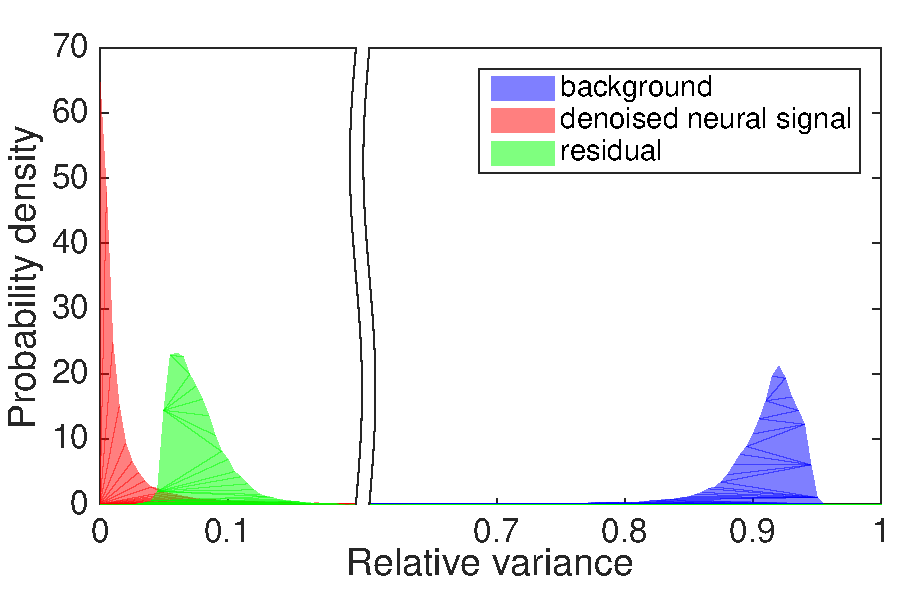
\includegraphics[height=1.62in]{Fig_Striatum_subfigs/variance_explained.pdf}}
\put(2.18, -1.59){\large\textbf{C}}
\put(3.07, -1.53){\scriptsize Explained Variance}

% \put(2.0, -0.9){\Large $=$}

\end{picture}
\end{document}
